
\chapter{Coupling strategy from the Navier-Stokes equations to the shallow water equations}
\chaptermark{Coupling strategy from the NS equations to the SW equations}
\label{coupling}


\section{Introduction}



The aim of this chapter is to explore the possibilities of coupling the presented shallow water models with the Navier-Stokes equations.
In this research, the developments of chapters \ref{eulerian_sw} and \ref{eulerian_bsq} are combined with a NS solver, and have been presented in \cite{maso2022b}. Having all the formulations within the same framework -FEM and implementation- ease the strategy. The first part of the staggered approach presented in chapter \ref{chapter_introduction}, an action triggering an event is modelled with the Navier-Stokes equations and the information is transferred to the SW domain. This first coupling is applied to impulse waves generated by landslides.

\emph{Landslide Generated Waves} (LGW) are caused by a landslide impacting a water reservoir. LGW events can have devastating effects on the coastal areas of water basins, such as lakes, fjords and artificial reservoirs. 
The fjord district of western Norway is one of the zones of the world most affected by this major natural hazard \cite{hermanns2014catalogue}. Historical records over the last 400 years show that Norway has experienced at least two major LGW events every century \cite{Harbitz2014}. Only in the first half of the last century, the catastrophic events of Loen (in 1905 and 1936) \cite{grimstad1991loen} and Tafjord (in 1934) \cite{higman20182015} caused the death of 174 people. The LGW events of Lituya Bay, Alaska, in 1958 \cite{Miller1960} and Vajont, Italy, in 1963 \cite{Semenza1965} are among the most well-known cases of this cascading natural hazard.
A wider overview of LGW historical events can be found in \cite{roberts2014preliminary}.
Furthermore, this situation is made even more critical by the effects of global warming, which is clearly leading to an increment in number and intensity of natural disasters \cite{Haque2019}.

In this new strategy, the Particle Finite Element Method (PFEM) \cite{idelsohn2004, onate2004, cremonesi2020state}, is used as the NFS and a the Boussinesq model presented in chapter \ref{eulerian_bsq} is used as the FFS. Several previous works have shown the accuracy of the PFEM to model landslides \cite{PFEMzhang1, PFEMzhangLandslide, zhang2021gpu}, also in cascading events \cite{CremonesiPFEM2, Salazar2012, CremonesiSlipLandslides, ZhangSubmarine}. In this work, we use the PFEM approach that has been successfully applied to LGW scenarios in \cite{mulligan2020} and in \cite{franci20203dA, franci20203dB}, where 3D simulations of the Vajont disaster were presented. This work aims at being a proof of concept of this new coupled strategy for real LGW scenarios. For this reason, a deep validation of the method is presented by analyzing the performance and accuracy of the new partitioned technique in targeted tests, using reference solutions obtained with other numerical methods, experimental tests and analytical solutions. In partitioned methods, the momentum transfer between the Navier-Stokes and the Boussinesq models must be accurate in order to obtain a faithful representation of the LGW scenario.
Thus, particular attention is devoted here to analyze the effect of the near-field boundary conditions on the far-field propagating wave. Convergence and sensitivity analyses are carried out in order to verify the accuracy and robustness of the proposed method.

In this chapter, after explaining the staggered strategy, it is analyzed in detail. Three examples are provided in order to validate the proposed partitioned strategy and to show its potential to large-scale LGW events.





\section{Coupling strategy}


The LGW problem is here simulated using a weakly coupled (one-way) method which makes interact the PFEM solver presented in Section \ref{state_art}, and the SW solver described in Chapters \ref{eulerian_sw} and \ref{eulerian_bsq}. 

We note that problem (\ref{bsq_eq}) defines a phase speed $c$ which in the SW limit is computed as $\sqrt{gh}$. Being $u$ the modulus of the horizontal velocity $\mathbf{u}_\beta$, the information travels at velocities $u+c$ and $u-c$. If the flow is subcritical, which is the case analyzed in this work, then $u<c$ and the information travels both upstream and downstream.

Considering the bidirectional characteristics of the equations, a first possibility would be to consider two domains adjacent to each other and define a strong (two-way) coupling (see for example \cite{pringle2016}).
However, such a strongly coupled approach is computationally expensive, as it requires running parallelly the PFEM and the SW solvers. 

Moreover, the accuracy increment given by a two-way method over a one-way strategy on the far-field wave propagation can be considered negligible. For these reasons, here, we adopt a decoupled space-time one-way strategy in which the PFEM solution is stored at the SW interface and, in a second stage, it is imposed as a boundary condition for the SW simulation. In order to avoid perturbations of the results at the interface, the computational domain of the PFEM is extended beyond the position of the SW interface using non-reflecting boundaries.



\begin{figure} [htb]
    \begin{subfigure}{\textwidth}
        \centering
        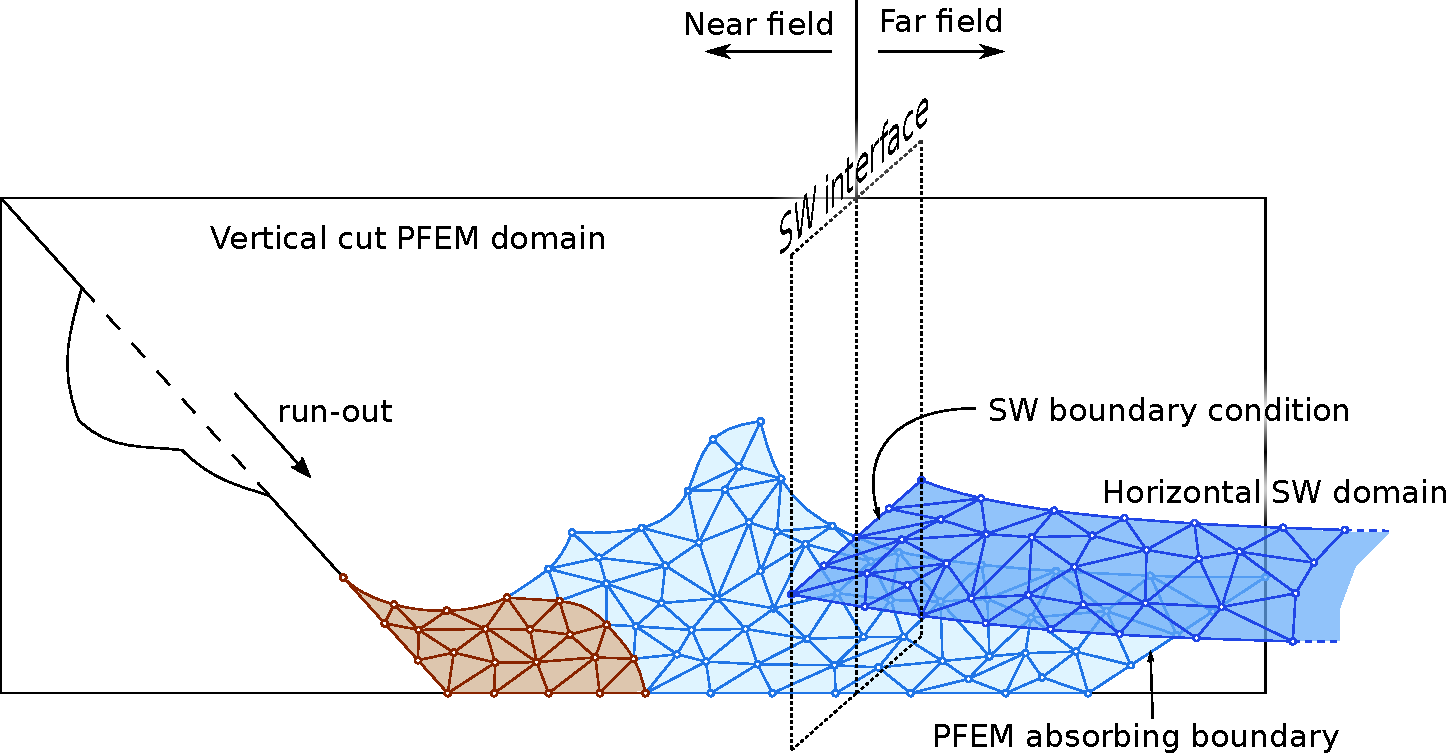
\includegraphics[width=\columnwidth]{img/coupling/modelView.pdf}
        \caption{Scheme of a 2D-PFEM-SW coupled strategy.}
        \label{coupling_model_simplified}
        \vspace{1em}
    \end{subfigure}
    \begin{subfigure}{\textwidth}
        \centering
        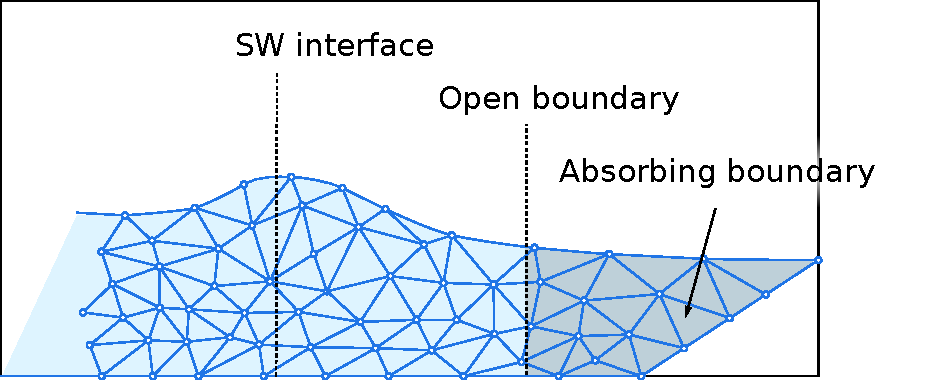
\includegraphics[width=\columnwidth]{img/coupling/open_boundary.pdf}
        \caption{Detail of the open boundary.}
        \label{coupling_model_boundary}
    \end{subfigure}
    \caption{Schematic view of the $near$-$field$ $solver$ and the $far$-$field$ $solver$ for the coupled solution of LGW.}        
    \label{coupling_model_scheme}
\end{figure}



Taking advantage of such a one-way coupling strategy, the PFEM and SW simulations can be executed independently leading to a very versatile tool for LGWs with significant saves of computing time.
Since the PFEM is a Lagrangian strategy, a search algorithm is constructed at every time step in order to find all the elements cut by the SW interface.
Then, the PFEM calculations beyond the interface are not relevant. This fact is the key to the computational savings, since the computational domain can be shortened by means of an open boundary. However, the numerical approximation of open boundaries --the absorbing boundaries-- introduces some reflections. In this work, the absorbing boundary is 
modelled by extending the domain after the open boundary with a gentle slope. The computational domain ends when the slope reaches the mean water level, at this point, the impulse waves leave the computational domain.

In a later stage, the characteristic variables computed at the interface are imposed to the SW domain through an inflow boundary condition. We recall the subcritical characteristics of the analyzed flows, hence, one variable is required to be imposed in order to define a well-posed problem: the wave amplitude or the horizontal velocity. 
We choose to impose the velocity, since it is more representative of the momentum exchange from the PFEM and the SW computation. It has proven to be accurate, even when the Boussinesq assumptions are not perfectly fulfilled.
A general picture of the coupling strategy is illustrated in Fig. \ref{coupling_model_scheme}.

Even though the Boussinesq equations are expressed in terms of the velocity evaluated at a certain depth, $\mathbf{u}_\beta$, this magnitude is a measure of the depth-averaged velocity $\bar{\mathbf{u}}$. In other words, it can be understood as a numerical quadrature of one integration point. When the waves are regular, the choice of one magnitude or another is not relevant, but when wave breaking is present, the depth-averaged velocity is more representative of the momentum exchange.
%An interesting property of the mean velocity is its robustness when dealing with a flux that is not fully developed. Indeed, the mean velocity represents a very good measure of the momentum exchange.

We remark that the average vertical velocity of the fluid corresponds to the time derivative of the free surface elevation. This variable does not correspond to a boundary condition for the studied cases.

Finally, there is an additional condition associated to $\Gamma_I$ (see Chapter \ref{eulerian_bsq}): the dispersive field $\mathbf{J}_\eta$ relates $\bar{\mathbf{u}}$ and $\mathbf{u}_\beta$. The assumption of equal velocities is equivalent to imposing $\nabla\nabla\cdot\mathbf{u}=\mathbf{0}$.



\section{Examples}



%%%%%%%%%%%%%%%%%%%%%%%%%%%%%%%%%%%%%%%%%%%%%%%%%%%%%%%%%%%%%%
%%%%%%%%%%%%%%%%%%%%%%%%%%%%%%%%%%%%%%%%%%%%%%%%%%%%%%%%%%%%%%

In this section, three different cases are presented. These examples are selected to validate the partitioned strategy and to show its potential for practical applications. The first numerical example is aimed at reproducing a unidirectional wave generated in a laboratory channel. For this test, we carry out a detailed validation of the coupled method paying special attention to the transmission of boundary conditions between the near- and the far-field solvers. The simplicity of this test allows us to compare our results with both experimental measures and analytical solutions, and also with the numerical solution obtained with a full PFEM model. In the second example, we apply the partitioned method to a more representative example of LGW problems.  In this test, we reproduce numerically the water wave generated experimentally by the impact of a second mass of water sliding at high velocity over a steep slope. The last test aims at showing the applicability of the method to real-world LGW problems. For this purpose, we considered a realistic configuration of a LGW event occurring in an alpine lake. Our numerical solution is compared to another LGW solver presented in the literature.



\subsection{Solitary wave in a channel}
\label{Example1}

In this test, we reproduce the laboratory experiment carried out at a large wave flume of the Coastal Research Center in Hannover. A solitary wave is generated by a piston-type maker and travels 180m until reaching the final inclined slope. A schematic view of the wave flume is depicted in Fig \ref{solitary_wave_channel}. More details about the experiment can be found in \cite{krautwald2020,krautwald2022,krautwald2021}.

\begin{figure} [htb]
    \centering
    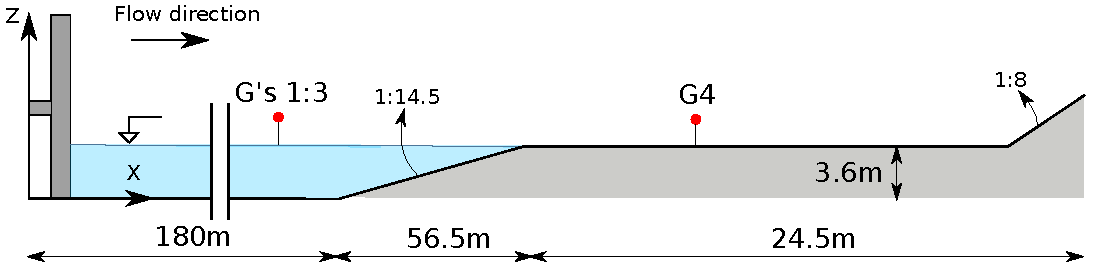
\includegraphics[width=\textwidth]{img/coupling/solitary_wave_channel.pdf}
    \caption{Solitary wave example. Schematic side view of the experimental flume studied. Units in m. Approximate position of the different wave gauges are also depicted.}
    \label{solitary_wave_channel}
\end{figure}

Fig. \ref{piston_stroke} shows the horizontal stroke of the paddle along time. The wave height has been monitored at different positions of the flume, including the on-shore zone. In this work, we will compare our numerical solution to the experimental measures obtained at the four wave gauges whose coordinates are given in Table \ref{solitary_wave_gauges_positions}. The selected gauges are placed at key positions of the channel and allow us to monitor wave generation (G1), propagation (G2), shoaling (G3) and flooding (G4).
%The fluid height level has been constantly monitored by Krautwald et al. in several positions of the wave flume. The studied wave gauges were placed offshore (WG8-14), in the slope (WG15) and in the channel platform (US4 and US5). In the present work, only the offshore wave height gauges are considered. The coordinates of each of the gauges are given in Table \ref{solitary_wave_gauges_positions}.


\begin{table} [htb]
    \begin{minipage}[b]{.48\textwidth}
    \centering
    \begin{tabular}{cc}
        \hline
        Gauge & Position [$m$] \\ \hline
        G1    &  60.0 \\
        G2    & 170.0 \\
        G3    & 223.5 \\
        G4    & 239.7 \\ \hline
    \end{tabular} \vspace*{20pt}
    \caption{Solitary wave example. Position of the different gauges in the flume.\\}
    \label{solitary_wave_gauges_positions}
    \end{minipage}
    \hfill
    \begin{minipage}[b]{.48\textwidth}
    \centering
    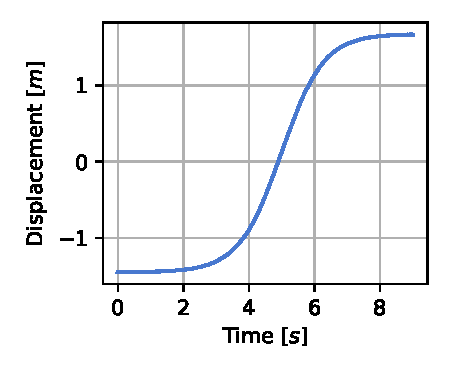
\includegraphics[width=.9\textwidth]{img/coupling/piston_stroke.pdf} \vspace*{-10pt}
    \caption{Solitary wave example. Paddle position according to time. Data provided in Krautwald et al. \cite{krautwald2020,krautwald2021,krautwald2022}.}
    \label{piston_stroke}
    \end{minipage}
\end{table}

\subsubsection{Physical considerations}


The aforementioned specifications generate a solitary wave of $0.6m$ amplitude and $65m$ wavelength. The wave generation, propagation and breaking were analyzed using the PFEM approach reported by Oñate et al. \cite{onate2022}.
Given the properties of such a solitary wave, it can be simulated using the Boussinesq approximation and thus reducing drastically the computational demand.
This experiment is very interesting for two reasons. Firstly, we can perform a verification test of both formulations and compare the numerical results against experimental data.
Secondly, the simplicity of the geometry allows us to obtain analytical solutions for the Boussinesq equations.
The analytical solution is a wave equation of the type
\begin{equation*}
\begin{split}
    u &= A_0 \text{sech}^2\phi \\
    \eta &= A_1 \text{sech}^2\phi + A_2 \text{sech}^4\phi
\end{split}
\end{equation*}
where $\phi=kx-\omega t$. Details of the parameters $A_0$, $A_1$ and $A_2$ and the relation between the wavelength, period and amplitude can be found in \cite{wei1995}.


The generation of solitary waves has motivated several discussions and a review can be found in \cite{guizien2010}.
The kinematic description of the piston wave maker is the origin of the discussion, since it cannot represent the exact solution of a solitary wave due to construction limitations.
Some expressions for the motion of the piston can be obtained by integrating the analytical solution of the wave and truncating it on a finite space and time domain, corresponding to the features of the piston. Then, the experimental solitary wave is generated with a tail of secondary oscillations.

The Lagrangian formulation of PFEM perfectly tracks the movement of the paddle and thus the numerical simulation reproduces the experimental results with high fidelity. On the other hand, since the Boussinesq equations are implemented in an Eulerian frame, this boundary condition is difficult to impose. An easier alternative is to apply the analytical solution as a boundary condition.

Fig. \ref{solitary_wave} shows the comparison between the solitary wave propagation obtained with the PFEM, the experimental results, and the Boussinesq and analytical solutions. The Boussinesq simulation shows no secondary oscillations because the solitary wave has been imposed perfectly. The PFEM analysis matches the experimental data and the SW analysis matches the analytical solution. The analytical solution overestimates the phase speed and this mismatch will be reflected in the following analyses. 

We remark that the difference in the phase speed of the wave is not originated by the coupling strategy, but by the Boussinesq approximation. The accuracy of the approximation depends on the non linearity ratio $\epsilon = \eta/H$ and dispersion ratio $\mu = H / \lambda$. A more detailed study can be found in \cite{wu2018}, particularly when $\epsilon<0.4$.


\begin{figure} [htb]
    \centering
    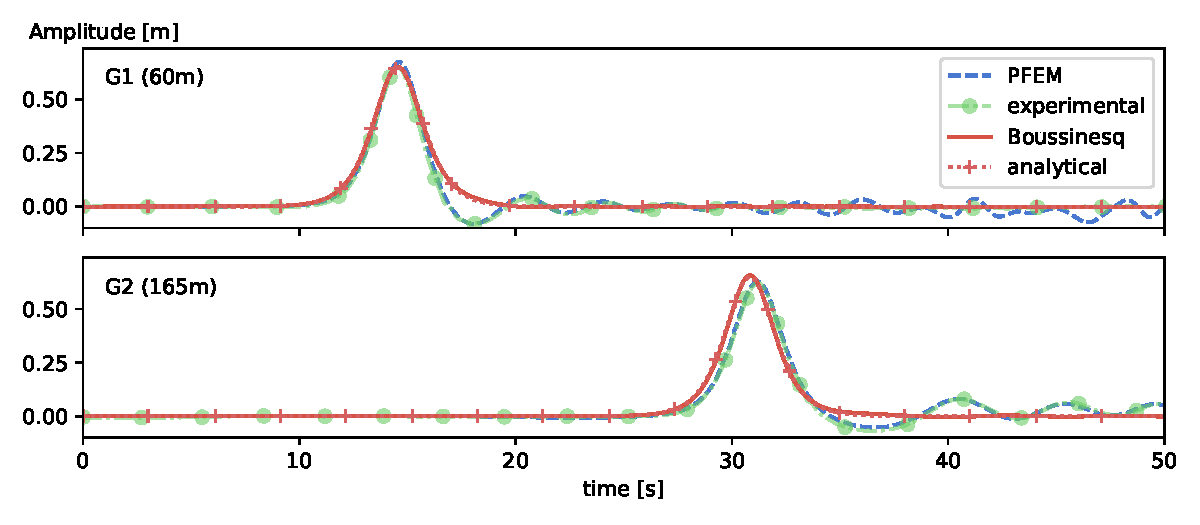
\includegraphics[width=\textwidth]{img/coupling/solitary_wave.pdf}
    \caption{Solitary wave example. Time evolution of the free surface at two gauges.}
    \label{solitary_wave}
\end{figure}



\subsubsection{Numerical results of the coupled strategy}

A global representation of the wave propagation is found in Fig. \ref{solitary_wave_propagation}. In this simulation, the first $10m$ are simulated using the 2D PFEM and the rest of the channel is simulated using the SW solver. Additionally, the full channel has been simulated with the PFEM to provide a reference solution for the coupled method and to analyze better its performance. Concerning the space and time discretizations used in the two solvers, the PFEM domain has a mesh of mean size $\Delta x=0.3m$ and the time step increment $\Delta t=0.001s$ is used, while the SW domain is discretized with $\Delta x=0.8m$ and $\Delta t=0.025s$.

\begin{figure} [htb]
    \centering
    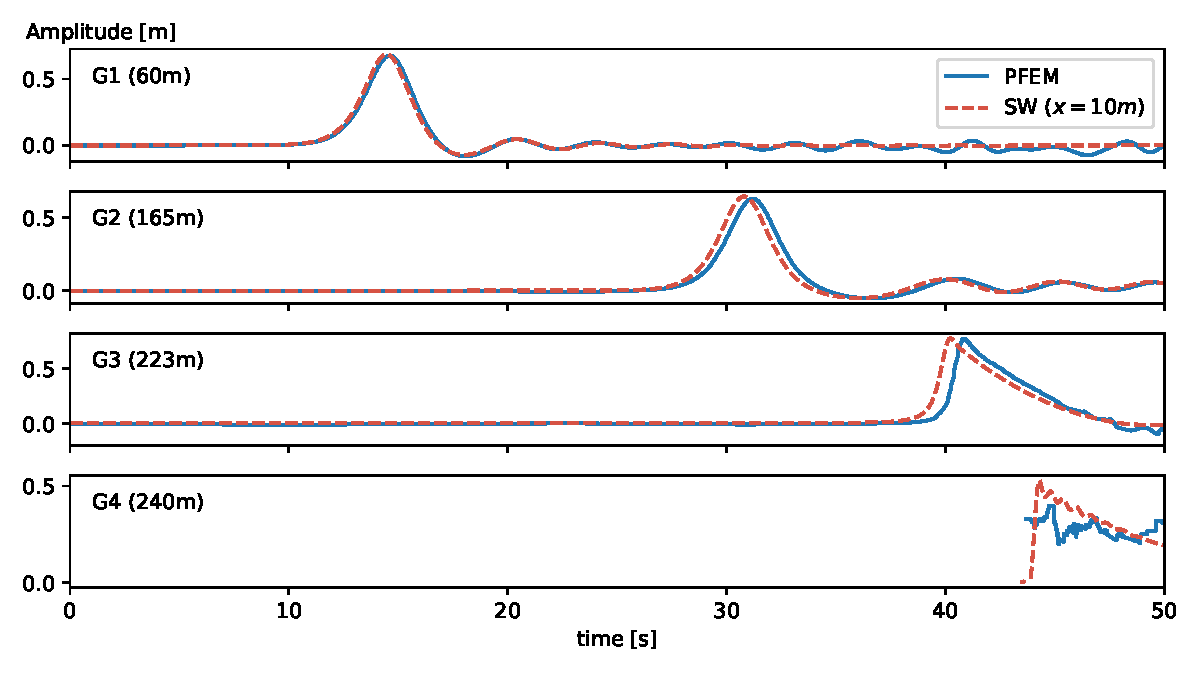
\includegraphics[width=\textwidth]{img/coupling/solitary_wave_propagation.pdf}
    \caption{Solitary wave example. Time series obtained with the interface at $x=10m$.}
    \label{solitary_wave_propagation}
\end{figure}

The results of gauges G2 and G3 show a small gap between the predicted wave by the two solvers. The Boussinesq approximation is triggering this gap, originated by an overestimation of the phase speed. This difference is consistent with wave theory and the current wave specifications. Note that the same gap can be observed in Fig. \ref{solitary_wave}.
The run-up (G4) is out of the SW theory assumptions, but still relevant results are obtained.

The magnitude of the computational time saving of the coupled method versus the full PFEM solution is about $95\%$. These savings will be analyzed in more detail in the next paragraphs. The savings depend on the spatial and temporal domain chosen for the NFS, that have to be carefully designed in order not to introduce additional errors.

%\subsubsection{Discussion of the coupling strategy}


%The coupling strategy has been tested with different configurations of the NFS and FFS. There is a 2D simulation of the full channel and some partial domains of $10$, $20$ and $30m$ length plus an extension acting as an absorbing boundary condition (see Fig. \ref{solitary_wave_pfem_meshes}). The partial simulations have been simulated using the 2D and 3D solver and the temporal domains are of $10$, $20$, $30$ and $40s$.

%\begin{figure} [htb]
%    \centering
%    \includegraphics[width=\textwidth]{img/solitary_wave_pfem_meshes.png}
%    \caption{Solitary wave example. (a) Detail of the full mesh of the channel, $20\,000$ elements. (b) The mesh with interface at $20m$, $3\,800$ elements. (c) The mesh with interface at $10m$, $2\,700$ elements.}
%    \label{solitary_wave_pfem_meshes}
%\end{figure}

%The FFS sensitivity has been tested with some SW interface positions at $x_1=10,\ 20,\ 30$ and $40m$. The possible combinations of NFS and FFS specifications are analyzed in order to evaluate the errors and time saving introduced by the coupling.


%In this example, the coupling strategy is extensively tested. The influence of the boundary conditions, the position of the interface, the spatial and temporal domain of the PFEM simulation, as well as the domain size (2D or 3D) at the PFEM model are analyzed in the following paragraphs.

%The coupling strategy has been tested with different interface positions ($x_1=10,\ 20,\ 30$ and $40m$) and different configurations of the NFS.

%Several interfaces have been positioned at the coordinates $x_1=10,\ 20,\ 30$ and $40m$. Each interface corresponds to a different SW mesh. The PFEM 3D domain is discretized with $\Delta x=0.4m$ and $\Delta t=0.001s$, the 2D domain with $\Delta x=0.3m$ and $\Delta t=0.001s$. Some of the 2D PFEM meshes are depicted in Fig. \ref{solitary_wave_pfem_meshes} .The SW domain is discretized with $\Delta x=0.8m$ and $\Delta t=0.025s$.



%\paragraph{Influence of the velocity $\bar{\mathbf{u}}$ or $\mathbf{u}_\beta$}
%As stated in section \ref{SW_model}, the boundary conditions should be specified by the velocity at a fixed depth $\beta H$, but the depth-integrated value presents some interesting advantages, such as smoothing the turbulent or numerical oscillations.
%Table \ref{solitary_wave_BC_errors} presents the computed wave amplitude errors at different interfaces positions.
%It can be seen that imposing the velocity $\mathbf{u}_\beta$ has an error about $1\%$ and imposing the velocity $\bar{\mathbf{u}}$ about a $3\%$ error. However, it is difficult to correlate both velocities with a parameter. In the following sections, we will use the velocity $\bar{\mathbf{u}}$, sacrificing a little of precision for robustness.




\subsubsection{Sensitivity to the interface position}
The FFS sensitivity has been tested with some SW interface positions at $x_1=10,\ 20,\ 30$ and $40m$.
One would expect to obtain a more accurate response as the interface is placed further away from the paddle.
Nevertheless, since in this example the wave is very regular, the observed influence of the interface position on the results is not significant.
The solutions obtained with all the interfaces can be considered already converged (Table \ref{solitary_wave_BC_errors_interface}). These results were expected due to the regularity of the wave. For this reason, a similar study is also performed in Section \ref{Example2}, where the SW interfaces are placed into a more chaotic fluid flow.


\begin{table} [htb]
    \centering
    \begin{tabular}{cccc}
        \hline
\multicolumn{4}{c}{Interface position}  \\ \cline{1-4}
$10m$    & $20m$    & $30m$   & $40m$   \\ \hline
2.48\%   & 3.01\%   & 3.12\%  & 2.84\%  \\ \hline
    \end{tabular}
    \caption{Solitary wave example. Wave amplitude errors computed at gauge 3 ($x=170m$) for different positions of the SW interface. Reference solution: full PFEM simulation.}
    \label{solitary_wave_BC_errors_interface}
\end{table}


\subsubsection{Sensitivity to the temporal domain}
Part of the saving in computational time comes from reducing the duration of the PFEM simulation up to the minimum time needed. 
Once the initial impulse has generated the wave and it has been transferred to the SW domain, the PFEM computations do not provide relevant information. From that time on, the initial boundary condition, which corresponds to water at rest, is imposed at the SW domain.  

This transition in the BC has to be carefully treated in order to avoid unphysical oscillations. A good duration for the transition is half of the period of the current wave.

In this test, we evaluate the effect of feeding the FFS with NFS solutions limited in time. In particular, we considered four PFEM analyses of duration $10$, $20$, $30$, and $40s$.

Fig. \ref{solitary_wave_time_convergence} shows the time evolution of the wave amplitude at the first gauge. In the graph, we also added dots representing the time instant when one analysis starts to diverge from the rest. It is clearly observed that the four solutions have an identical behavior in the first part of the graph. In particular, even with just $10s$ of the PFEM simulation, the main wave is well reproduced. Beyond this time, the curves diverge progressively. As expected, a time interval of around 10 seconds separates the consecutive diverging points.

\begin{figure} [htb]
    \centering
    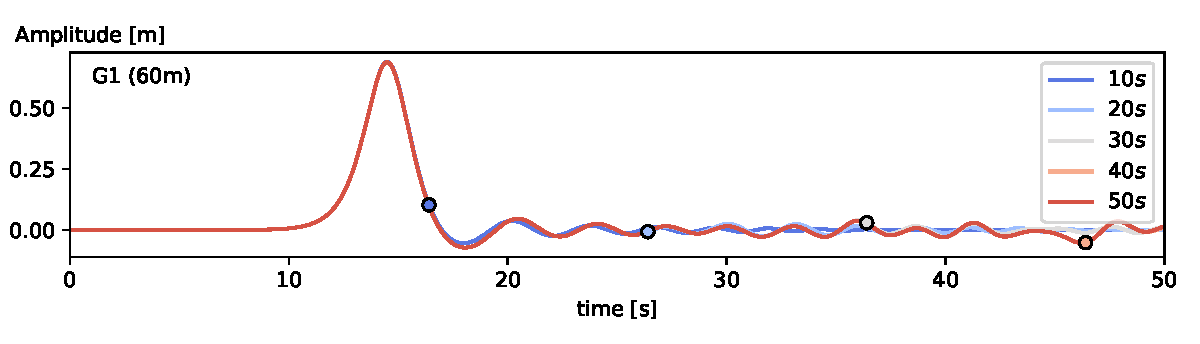
\includegraphics[width=\textwidth]{img/coupling/solitary_wave_time_convergence.pdf}
    \caption{Solitary wave example. Set of analysis where the interface is active only in a part of the time domain. The marker shows when the solution tends to the resting condition.}
    \label{solitary_wave_time_convergence}
\end{figure}




\subsubsection{Sensitivity to PFEM domain length}
Besides the reduction of the time duration of the analyses, the optimization of the size of the PFEM computing domain can drastically reduce the computational cost of the simulations without affecting the accuracy of the results.
For this reason, we analyze here the effect of considering partial PFEM domains of $10$, $20$ and $30m$ length plus an extension acting as absorbing boundary condition, as shown in  Fig. \ref{solitary_wave_pfem_meshes}. The study is carried out for both 2D and 3D PFEM domains.
\begin{figure} [htb]
    \centering
    \includegraphics[width=\textwidth]{img/coupling/solitary_wave_pfem_meshes.png}
    \caption{Solitary wave example. (a) The mesh with interface at $10m$, $2\,700$ elements. (b) The mesh with interface at $20m$, $3\,800$ elements. (c) Detail of the full mesh of the channel, $20\,000$ elements. The slope has a dissipative effect and is acting as an absorbing boundary.}
    \label{solitary_wave_pfem_meshes}
\end{figure}
%The accuracy of the wave propagation is studied under the generation of three PFEM domains. The channel has been shortened to $10$, $20$ and $30m$ and the reflections have been avoided with a shallow slope of $1:10$ (Fig. \ref{solitary_wave_pfem_meshes}).
The errors introduced by the effect of shortening the PFEM domain are listed in Table \ref{solitary_wave_partial_mesh_errors}.

\begin{table} [htb]
    \centering
    \begin{tabular}{c|ccc|ccc}
        \hline
        \multirow{3}{*}{\makecell{PFEM\\domain\\length}} &
        \multicolumn{3}{c|}{PFEM 2D} &
        \multicolumn{3}{c} {PFEM 3D} \\ \cline{2-7}
        &
        \multicolumn{3}{c|}{SW interface position} &
        \multicolumn{3}{c} {SW interface position} \\ \cline{2-7}
               &  $10m$    &  $20m$   &  $30m$   &  $10m$    &  $20m$   &  $30m$   \\ \hline
        $30m$  & -0.652\%  & -0.984\% & -6.37\%  &  0.228\%  &  -3.0\%  &  -7.16\% \\
        $20m$  & -0.635\%  & -5.97\%  &     -    & -0.438\%  & -5.62\%  &     -    \\
        $10m$  & -5.21\%   &    -     &     -    & -5.24\%   &    -     &     -    \\ \hline
    \end{tabular}
    \caption{Solitary wave example. Errors of the wave amplitude computed at gauge 3 ($x=170m$) with different configurations. Reference solution: coupled solution obtained with the full PFEM domain, as shown in Fig. \ref{solitary_wave_pfem_meshes}c.}
    \label{solitary_wave_partial_mesh_errors}
\end{table}

It is important to note that the vicinity of the absorbing boundary condition of the PFEM may affect the accuracy of the interface. The small errors obtained when the interface is far enough from the absorbing boundary show that the presented methodology allows to effectively reduce the PFEM domain without virtually affecting the quality of the solution.
This is particularly noticeable in the 2D case.


The 3D case presents a similar behavior, but higher errors are observed in the $30m$ domain length. 
%This is related to the difficulty of simulating this problem, where the boundary conditions -the walls of the channel- are very close. 
However, these errors are more attributable to the capabilities of the NFS for reproducing the fluid-solid interaction at the lateral walls (see \cite{onate2022} for more details) than to the coupling strategy. A finer discretization in the PFEM mesh would reduce this bias.


% \subsubsection{Conclusions}

% In this example, the error induced by the coupling strategy is analyzed. It can be decomposed into several components: the approximation of the Boussinesq equations, the boundary condition imposed at the SW interface, the absorbing boundary condition of the PFEM, and the temporal truncation of the PFEM temporal domain.
% \begin{itemize}
% \item The error associated with the Boussinesq approximation depends on the wave characteristics, usually, it is small since the LGW fulfills the physical assumptions. In this case, the error associated with the Boussinesq assumptions is of the order of 2\%.
% \item The error introduced by the specification of the velocity ($\bar{\mathbf{u}}$ or $\mathbf{u}_\beta$) at the SW boundary condition is not appreciable. Once the wave has propagated a wavelength, the possible differences have been dissipated due to the Boussinesq approximation. For robustness, we propose the use of the mean velocity.
% \item The truncation of the temporal domain of the PFEM analysis does not introduce errors once the LGW has trespassed the interface.
% \item The truncation of the spatial domain of the PFEM analysis is more sensitive since the absorbing boundary condition introduces some reflections. This is the major error associated with the coupling strategy. Selecting an interface far enough from the absorbing boundary is of crucial importance to keep the overall error of the order of the Boussinesq approximation.
% \item INFLUENCE OF PFEM 2D-3D...
% \end{itemize}




%%%%%%%%%%%%%%%%%%%%%%%%%%%%%%%%%%%%%%%%%%%%%%%%%%%%%%%%%%%%%%
%%%%%%%%%%%%%%%%%%%%%%%%%%%%%%%%%%%%%%%%%%%%%%%%%%%%%%%%%%%%%%

% \clearpage
\subsection{Wave generated by a water landslide}
\label{Example2}

In the second example, we simulate the experiment carried out at the Queen's University landslide flume presented in \cite{bullard2019}. In this laboratory test, a mass of water is released from an elevated reservoir and, after flowing downhill over a $30^\circ$ slope, it impacts at high velocity the water at rest placed on a $33.8m$-long channel. 
In the reference work \cite{bullard2019}, 41 experiments were presented covering a wide range of source volumes and reservoir depths. In \cite{mulligan2020}, a comparison of experimental and numerical results obtained for three different water depths in the channel is presented. In this research, we select the largest volume case ($0.45m^3$) and water depth ($0.60m$). 
Fig. \ref{landslide_wave_channel} shows the geometry of the experimental setup considered in this work.



\begin{figure} [htb]
    \centering
    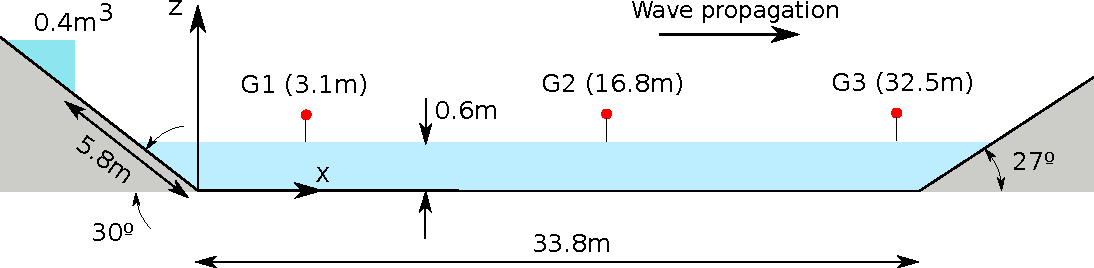
\includegraphics[width=\textwidth]{img/coupling/landslide_wave_channel.pdf}
    \caption{Landslide wave problem. Setup of the LGW flume for the experimental and numerical analyses.}
    \label{landslide_wave_channel}
\end{figure}



\begin{figure}[p]
    \def\imgoffset{15ex}
    \centering
    \begin{subfigure}[c]{\columnwidth}
        \caption{Runout ($t=0.7s$)}
        \centering
        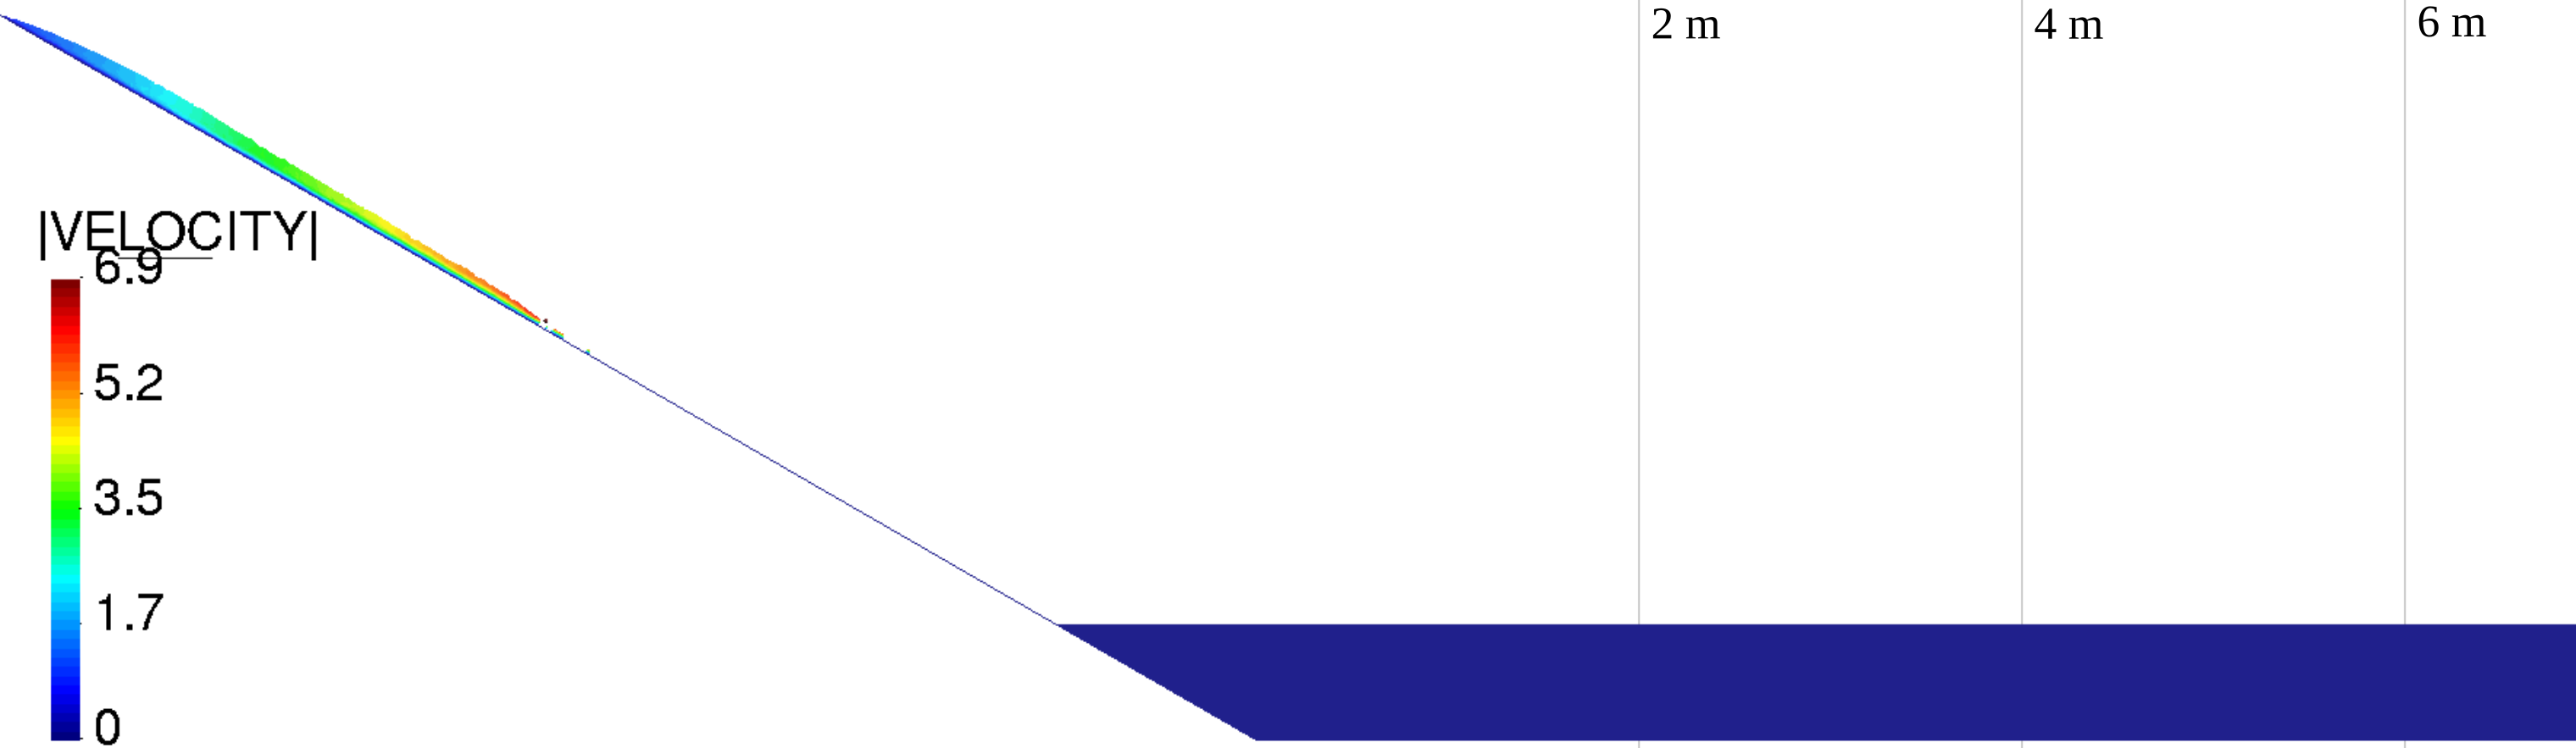
\includegraphics[width=\columnwidth]{img/coupling/t07.png}
        \label{t07pfemTest2}
    \end{subfigure}

    \begin{subfigure}[c]{\columnwidth}
        \caption{Impact ($t=1.5s$)}
        \centering
        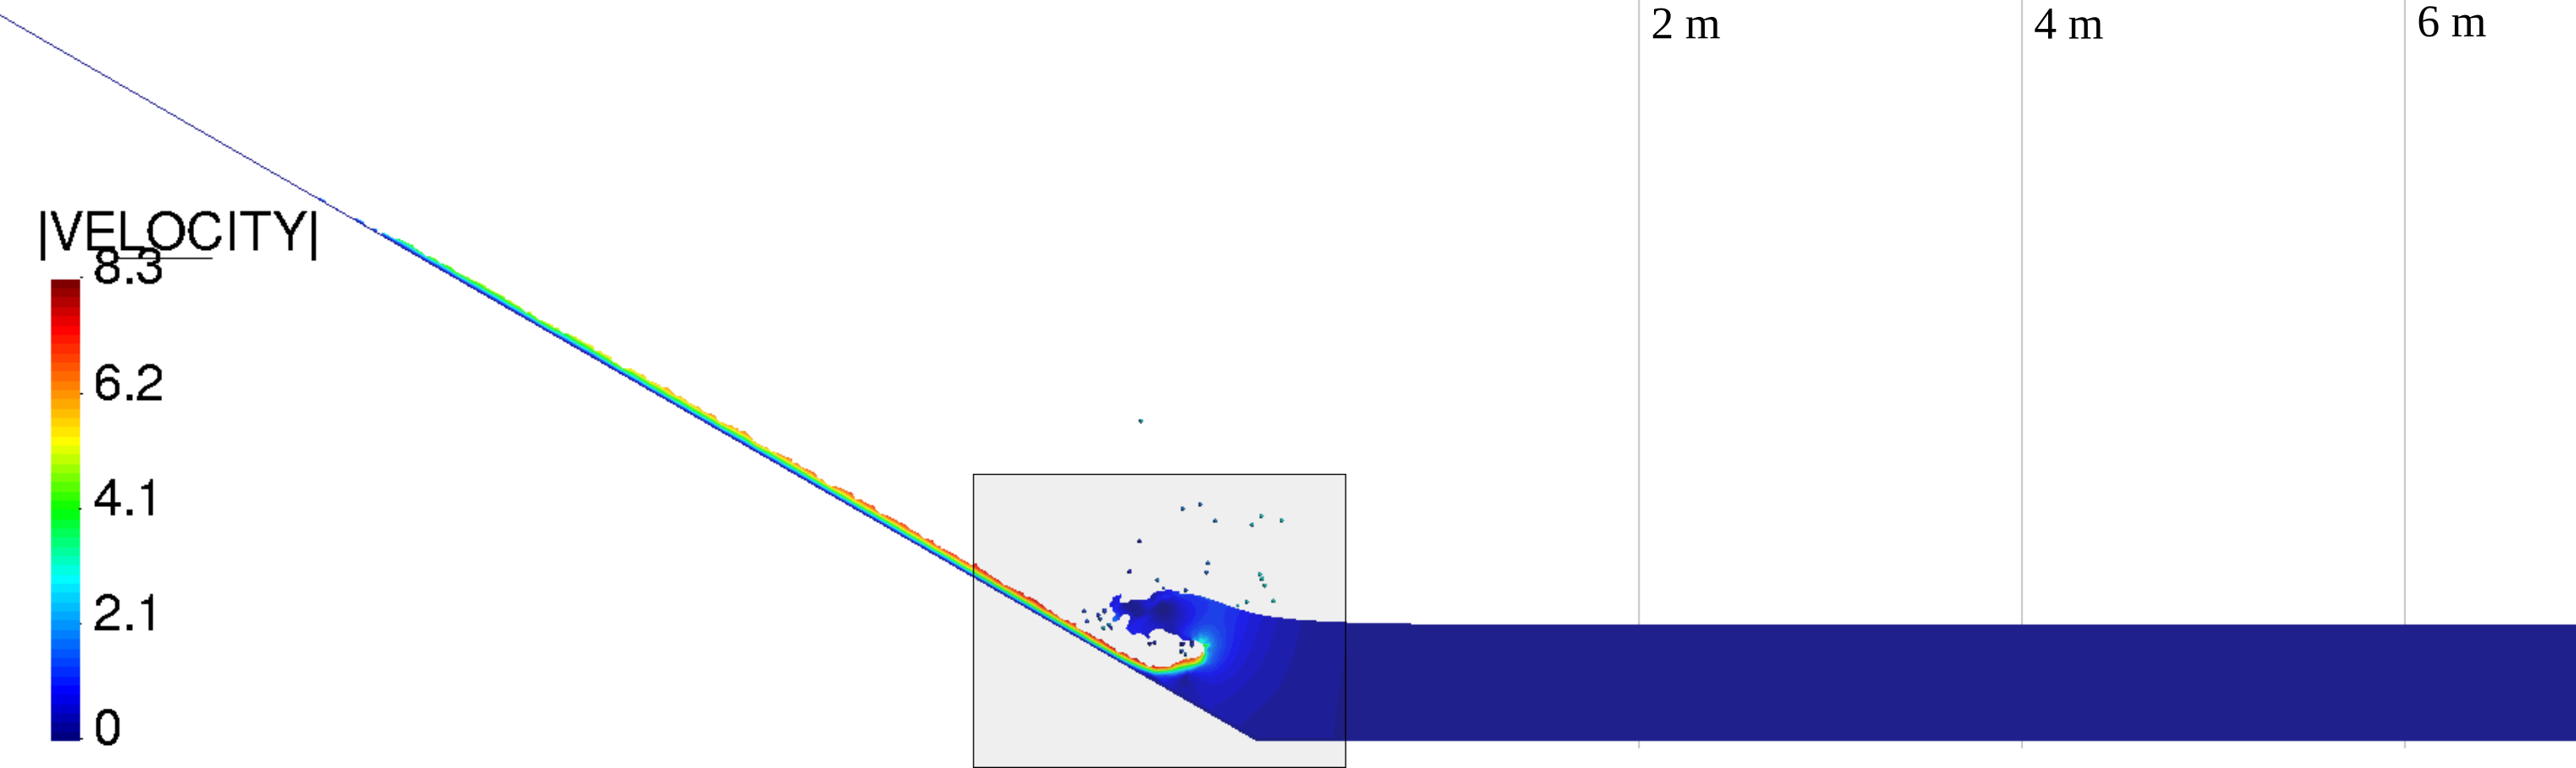
\includegraphics[width=\columnwidth]{img/coupling/t15.png}
        \label{t15pfemTest2}
    \end{subfigure}

    \begin{subfigure}[c]{\columnwidth}
        \centering
        \caption{Wave formation ($t=2.8s$)}
        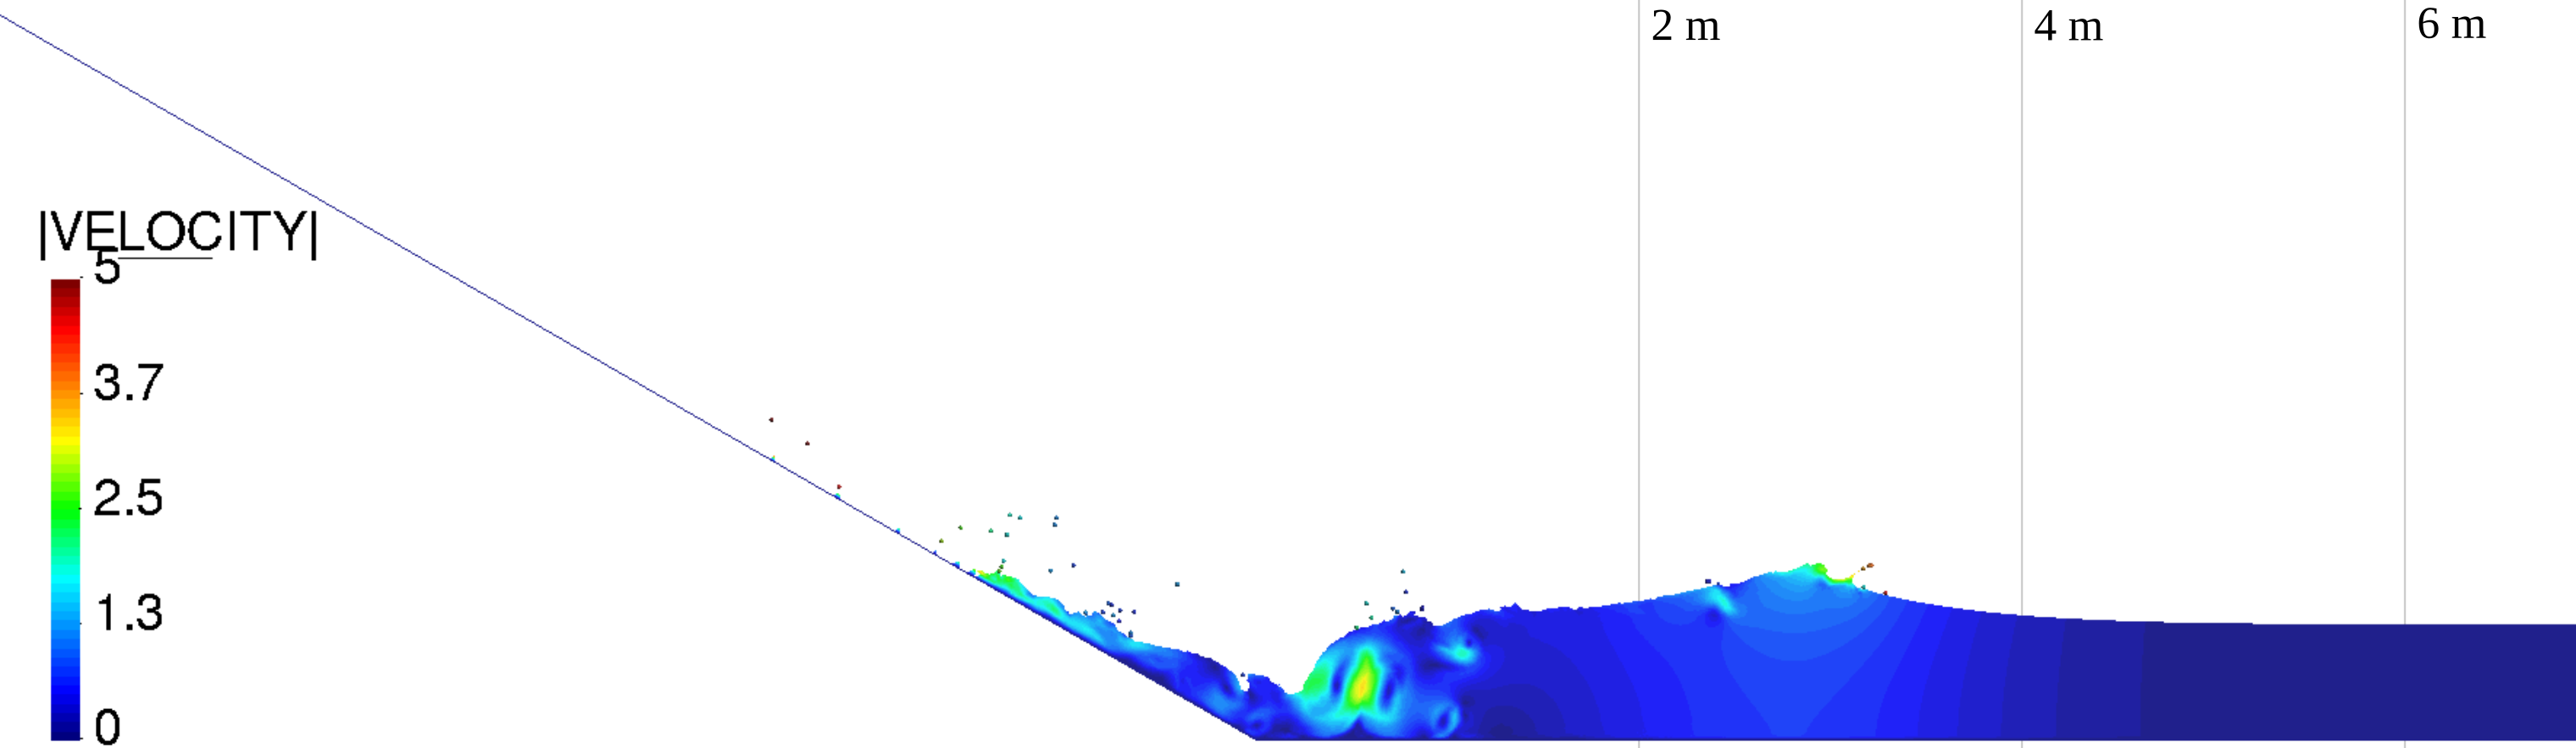
\includegraphics[width=\columnwidth]{img/coupling/t28.png}
        \label{t28pfemTest2}
    \end{subfigure}

    \begin{subfigure}[c]{\columnwidth}
        \centering
        \begin{minipage}[b]{0.35\textwidth}
            \caption{Impact zone modeled with the PFEM. Detail of Figure (b) adding the solving mesh. }
            \label{t07pfemTest2Zoom}
        \end{minipage}
        \begin{minipage}[c]{0.4\textwidth}
            \includegraphics[width=\textwidth]{img/coupling/t15zoom.png}
        \end{minipage}
    \end{subfigure}

    \caption{Landslide wave problem. Near-field results with the PFEM solution of Navier-Stokes problem. The thin vertical lines show the SW interfaces positions.}
    \label{PFEMresultsTest2}
\end{figure}


% \begin{figure} [h]
%     \centering
%     \includegraphics[width=0.7\textwidth]{img/t15zoom.png}
%     \caption{Landslide wave problem. Detail of Fig. \ref{t15pfemTest2} adding the solving mesh. Impact zone modeled with the PFEM. }
%     \label{t07pfemTest2Zoom}
% \end{figure}


We remark that considering a water landslide does not affect the relevance of the test in the field of LGWs. In fact, the phenomena produced by the water runout and impact are totally representative of a realistic LGW scenario with a fast mobilized material. Furthermore, the use of water as sliding material removes the uncertainty related to the rheological properties of the slide and allows repeatability of the test. 

The PFEM is used to simulate the water runout, the impact against the water at rest and the consequent wave formation (Fig. \ref{PFEMresultsTest2}). Remarkably, the front of the water landslide reaches the end of the slope with a thin layer of less than 10$cm$ and it impacts the water in the channel at a speed of about $10m/s$. Thus, in order to capture accurately the phenomena at the impact zone, a fine mesh and time discretizations are necessary. For this reason, a mesh size of $\Delta x=1.5cm$ and a time step increment of $\Delta t=5\cdot10^{-4}s$ are used in the PFEM simulations. 
On the other hand, a much coarser mesh and time discretizations can be used to model the wave propagation along the channel with the SW solver. In particular, in the FFS a time step of $\Delta t=0.025s$ and a mesh size of $\Delta x=0.3m$ have been used. We remark that the possibility of using much different and yet adequate space and time parameters in the FFS and NFS solvers is one of the main advantages of this partitioned method and one of the reasons for its high computational efficiency.



\subsubsection{Numerical results}

This LGW scenario has been solved using a time and space reduced PFEM domain in combination with three SW interfaces.
The PFEM spatial domain includes the runout, the first $7m$ of the flume and an absorbing boundary condition, while the temporal domain includes only the first $5s$.
The SW interfaces are positioned at $2,\ 4$ and $6m$. Fig. \ref{landslide_wave_propagation} presents the results obtained at the gauges and a representation of the wave propagation.

\begin{figure} [htb]
    \centering
    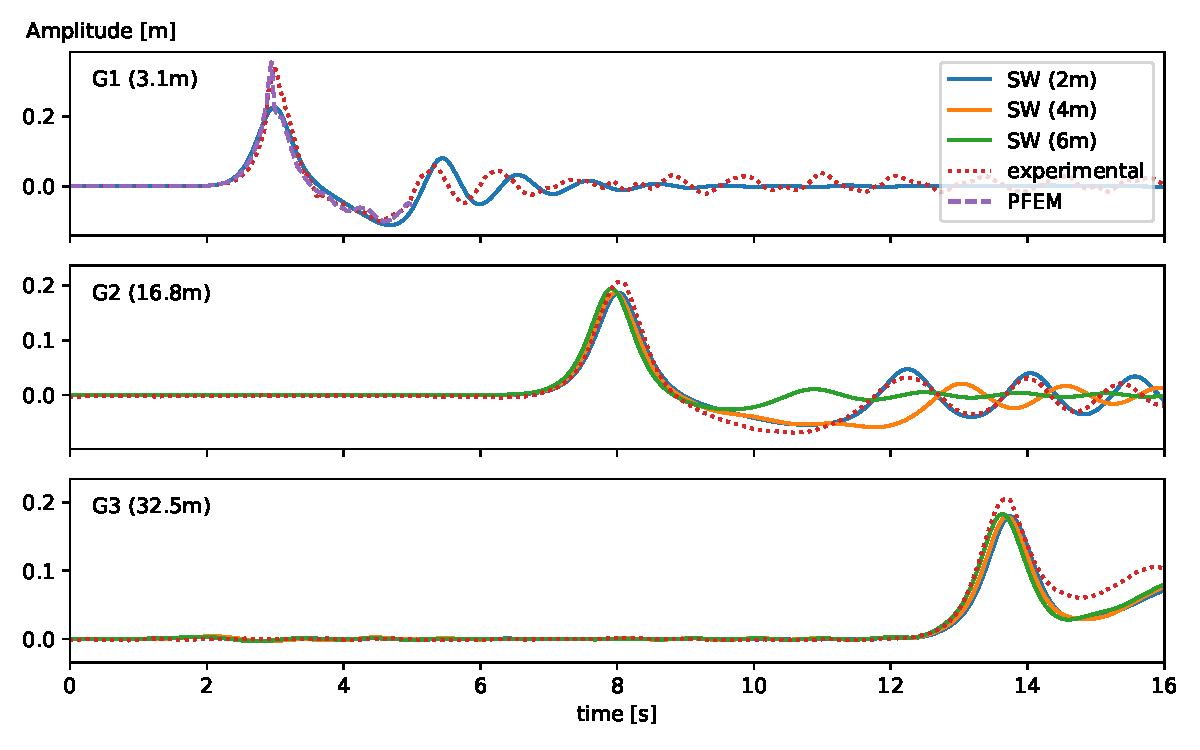
\includegraphics[width=\textwidth]{img/coupling/landslide_wave_propagation.pdf}
    \caption{Landslide wave problem. Time series of the wave amplitude at the different recording points.}
    \label{landslide_wave_propagation}
\end{figure}


In the top image, it can be observed the vicinity of the first gauge and the first SW interface to the wave generation zone. Indeed, gauge G1 can only record the PFEM solution and the SW solution obtained by the first interface. It is clear that the imposed boundary condition does not satisfy the Boussinesq assumptions and the interpolated wave does not fit the profile of a breaking wave.
However, although the wave interpolated by the FFS at the first stages is not equivalent in terms of wave height, the stored momentum is the correct one. This can be observed at gauges G2 and G3, where the experimental wave has adopted the solution of a solitary wave and matches the profile of the FFS.

The results obtained at gauges G2 and G3, placed at the middle and the end of the channel, respectively, show that all the three SW interface positions reproduce well the main wave obtained experimentally. This is particularly remarkable considering that the SW interface placed at $x=2m$ is completely inside the impact zone (Fig. \ref{PFEMresultsTest2}). These results show that, as long the momentum is well transferred from the NFS to FFS, the wave propagation process in the far-field can be accurately reproduced even considering the SW interface in a zone where the wave is not completely generated. We also remark that this can be done safely in this test, since water has been considered for the sliding material. In case of considering a different landslide material, either the interface is placed further the zone of material deposition of the landslide, or the interface boundary conditions have to take into account the presence of different materials in the computation of the overall momentum.

Gauge G2 also records a considerable time interval after the first wave, this allows us to analyze also the secondary waves. In this case, we note some discrepancies between the results obtained by three SW interface positions. In particular, the first solution that diverges from the experimental one (and from the two other numerical solutions) is that obtained by the farthest interface position ($6m$). This result is totally consistent with the time domain truncation explained in Example \ref{Example1} and Fig. \ref{solitary_wave_time_convergence}. As the interface position is further from the impact zone, the signal arrives later. Given the phase speed is about $2.5m/s$, the time difference between each interface is around $0.8s$.


As a concluding remark for this example, the computational cost of the full simulation of the LGW has been estimated proportionally to the time needed by the signal to arrive at the end of the channel and proportionally to the number of elements required to discretize the full domain. The resources consumed by the FFS can be neglected since they are two orders of magnitude smaller. According to these considerations, the overall time saving given by the proposed partitioned strategy is $95\%$.



%%%%%%%%%%%%%%%%%%%%%%%%%%%%%%%%%%%%%%%%%%%%%%%%%%%%%%%%%%%%%%
%%%%%%%%%%%%%%%%%%%%%%%%%%%%%%%%%%%%%%%%%%%%%%%%%%%%%%%%%%%%%%

% \clearpage
\subsection{Landslide in a representative alpine lake}
\label{Example3}

In \cite{app112411614}, different metrics of real alpine lakes were used to define the configuration of theoretical mountain basins of different sizes and shapes. These geometries were used in \cite{app112411614} to study LGW scenarios with a finite volume solver and to obtain correlations between the lake configuration and the landslide-generated waves. Here, we analyze one of the lakes considered in \cite{app112411614} to test the proposed coupled strategy in a 3D complex setup. 

Fig. \ref{lake_geometry} shows the side and top views of the geometry of the lake. 
The case study is a circular lake with a diameter of 1500 m. The landslide has a prismatic shape of $20$ $m$ thick, $208$ $m$ long and $120$ $m$ wide. Following \cite{app112411614}, a bulk material density of $1620$ $kg/m ^3$ is used for the landslide material and an initial velocity of $20$ $m/s$ has been prescribed to the sliding body.

\begin{figure}[ht]
    \centering
    \begin{subfigure}{0.6\textwidth}
        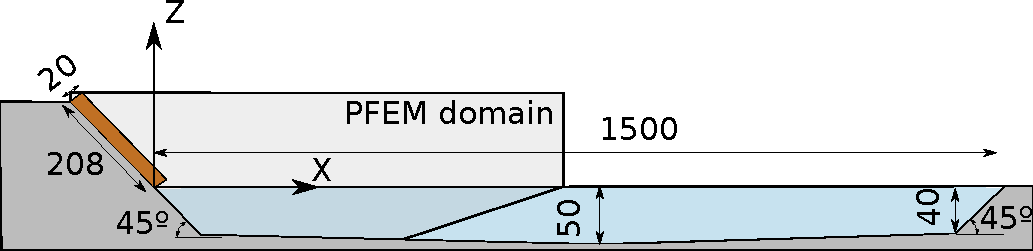
\includegraphics[width=\textwidth]{img/coupling/ex3_lateralview.pdf}
        \caption{Side view.}
        \label{ex3_lateralview}
    \end{subfigure}
    \par\medskip
    % \quad
    \begin{subfigure}{0.75\textwidth}
        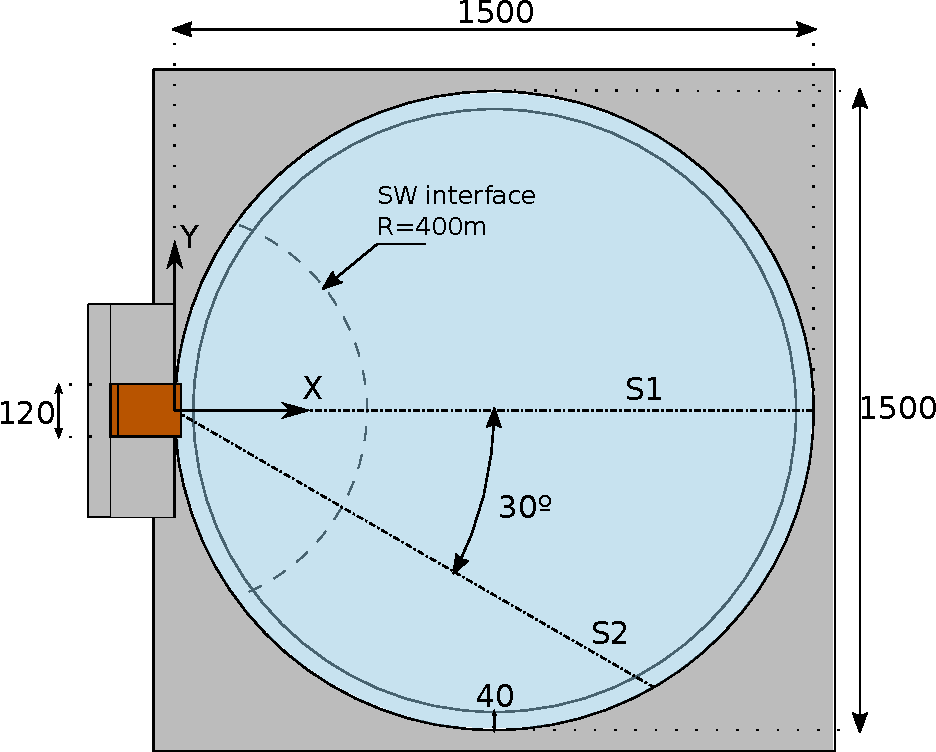
\includegraphics[width=\textwidth]{img/coupling/ex3_topview.pdf}
        \caption{Top view.}
        \label{ex3_topview}
    \end{subfigure}
    \caption{Landslide in a representative lake. Side and top view of the geometry. Dimensions in $m$.}
    \label{lake_geometry}
\end{figure}



Preliminary NFS analyses of the LGW scenario showed that the landslide material reaches a deposition distance of around $350m$. This information is useful to place the SW interface at a position that is not trespassed by the sliding material. For this reason, the interface of the FFS has been placed at $400m$ from the center of coordinates, which is the center of the run-out impact. 


\subsubsection{Numerical results}

Fig. \ref{ex3_postprocess} shows a global view of the simulated LGW and a superposition of the NFS and FFS results.


\begin{figure} [p]
    \centering
    % \def\svgwidth{\textwidth}
    % \input{img/ex3_drawing.pdf_tex}
    \begin{subfigure}{\textwidth}
        \centering
        \caption{Initial configuration ($t=0s$)}
        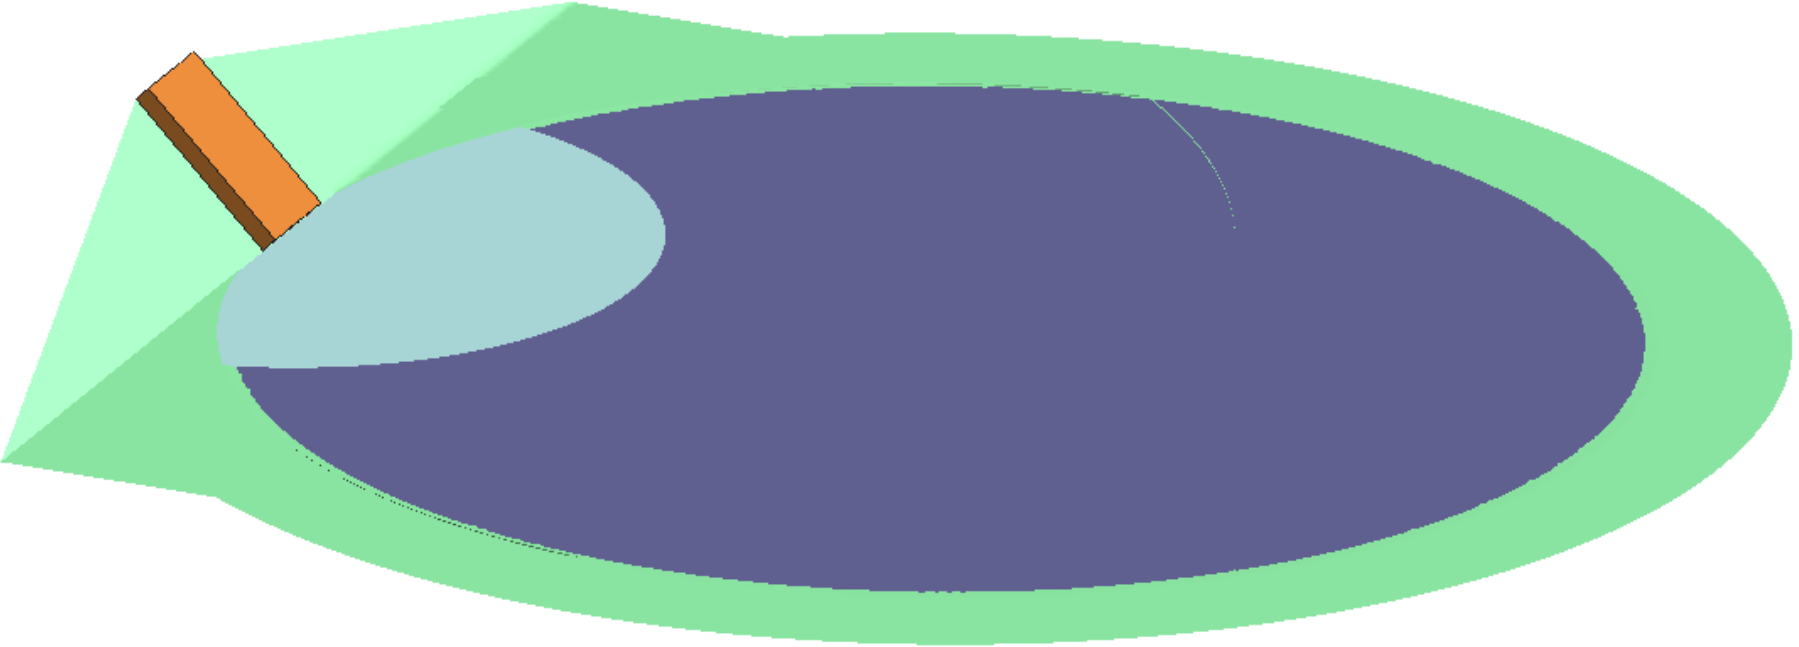
\includegraphics[width=.85\textwidth]{img/coupling/ex3_t0.png}
    \end{subfigure}
    \vspace{5pt}

    \begin{subfigure}{\textwidth}
        \centering
        \caption{Run-out and impact ($t=5s$)}
        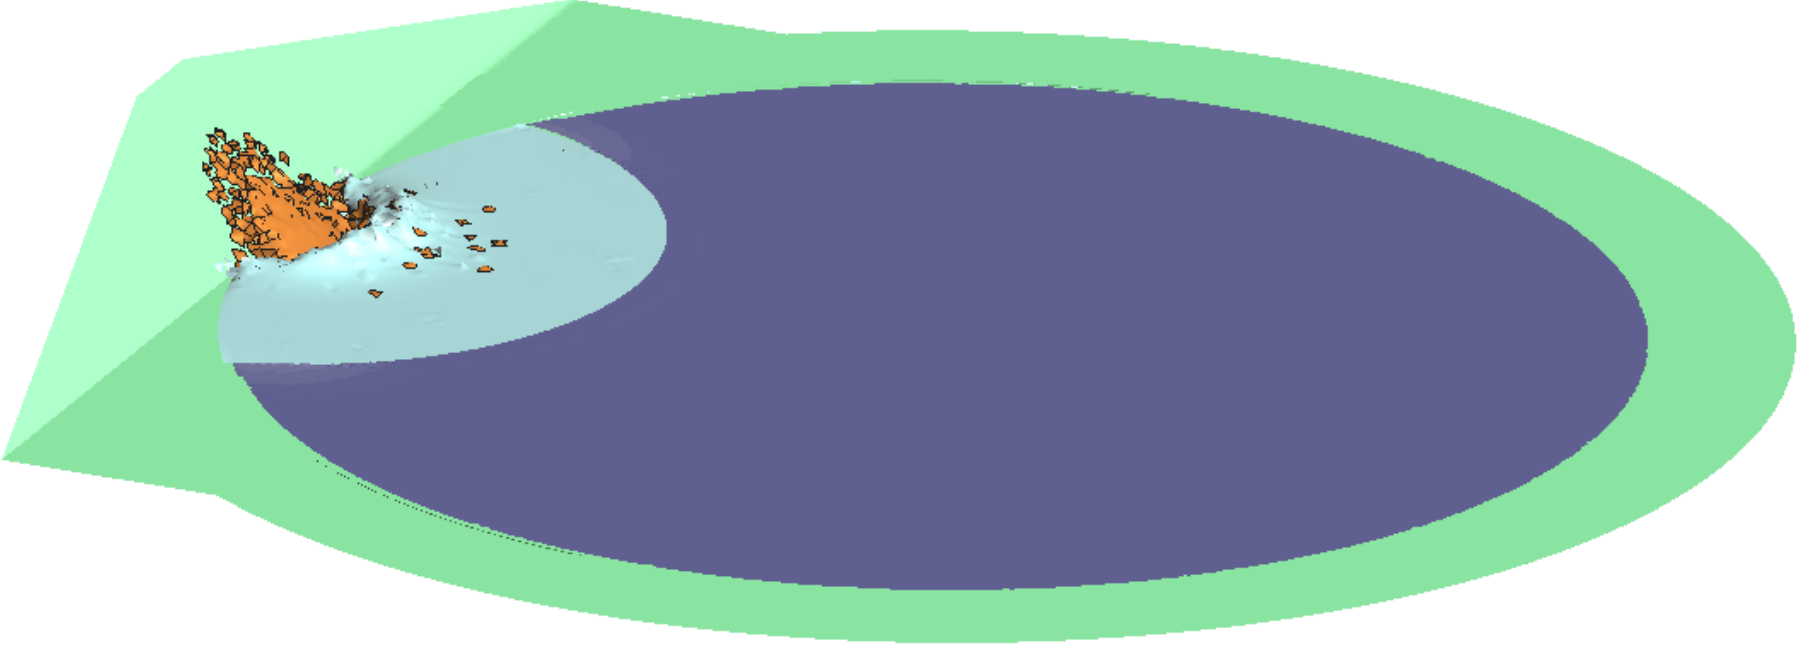
\includegraphics[width=.85\textwidth]{img/coupling/ex3_t5.png}
    \end{subfigure}
    \vspace{5pt}

    \begin{subfigure}{\textwidth}
        \centering
        \caption{Wave generation ($t=10s$)}
        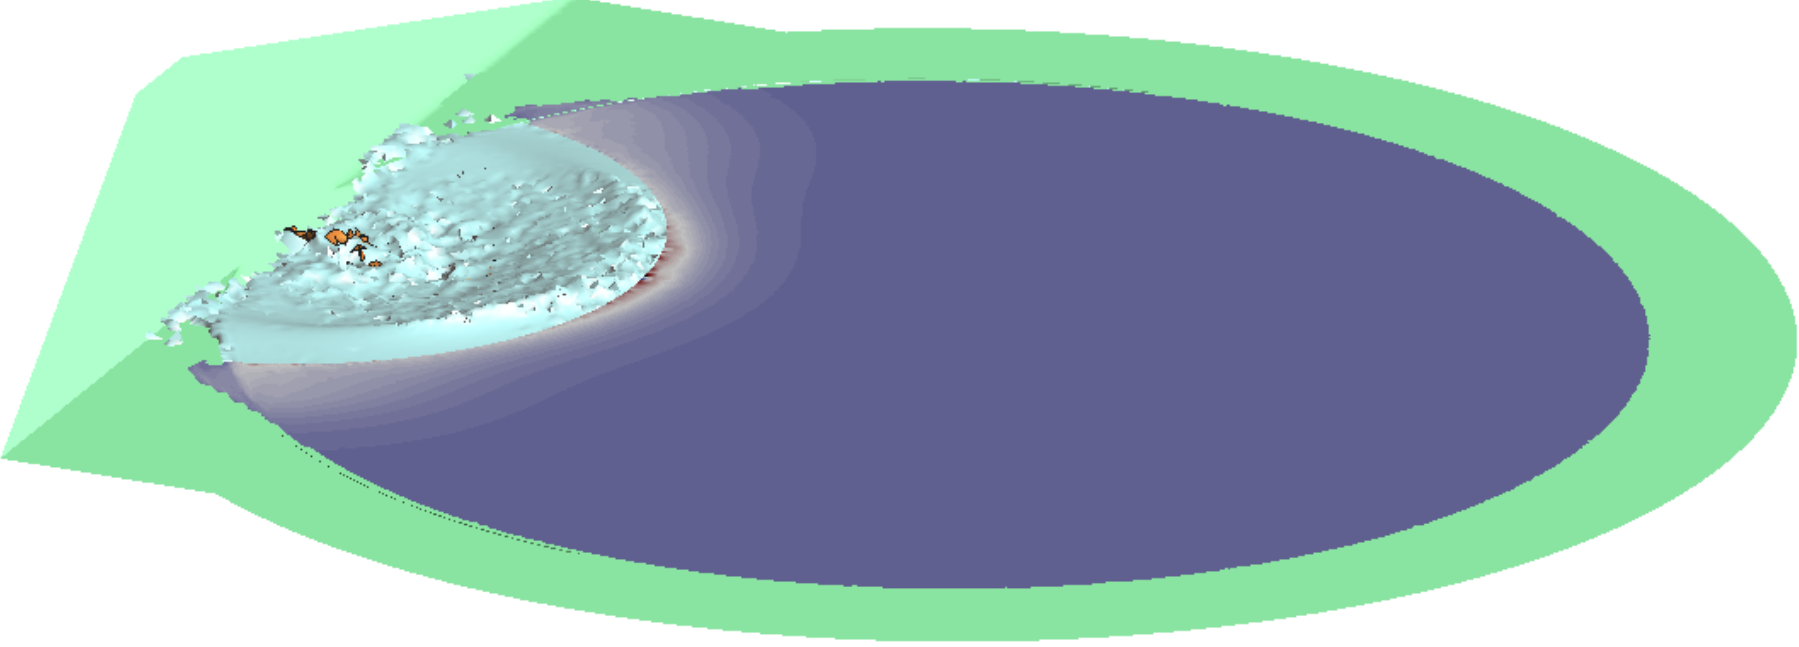
\includegraphics[width=.85\textwidth]{img/coupling/ex3_t10.png}
    \end{subfigure}
    \vspace{5pt}

    \begin{subfigure}{\textwidth}
        \caption{Wave propagation ($t=50s$)}
        \hfill
        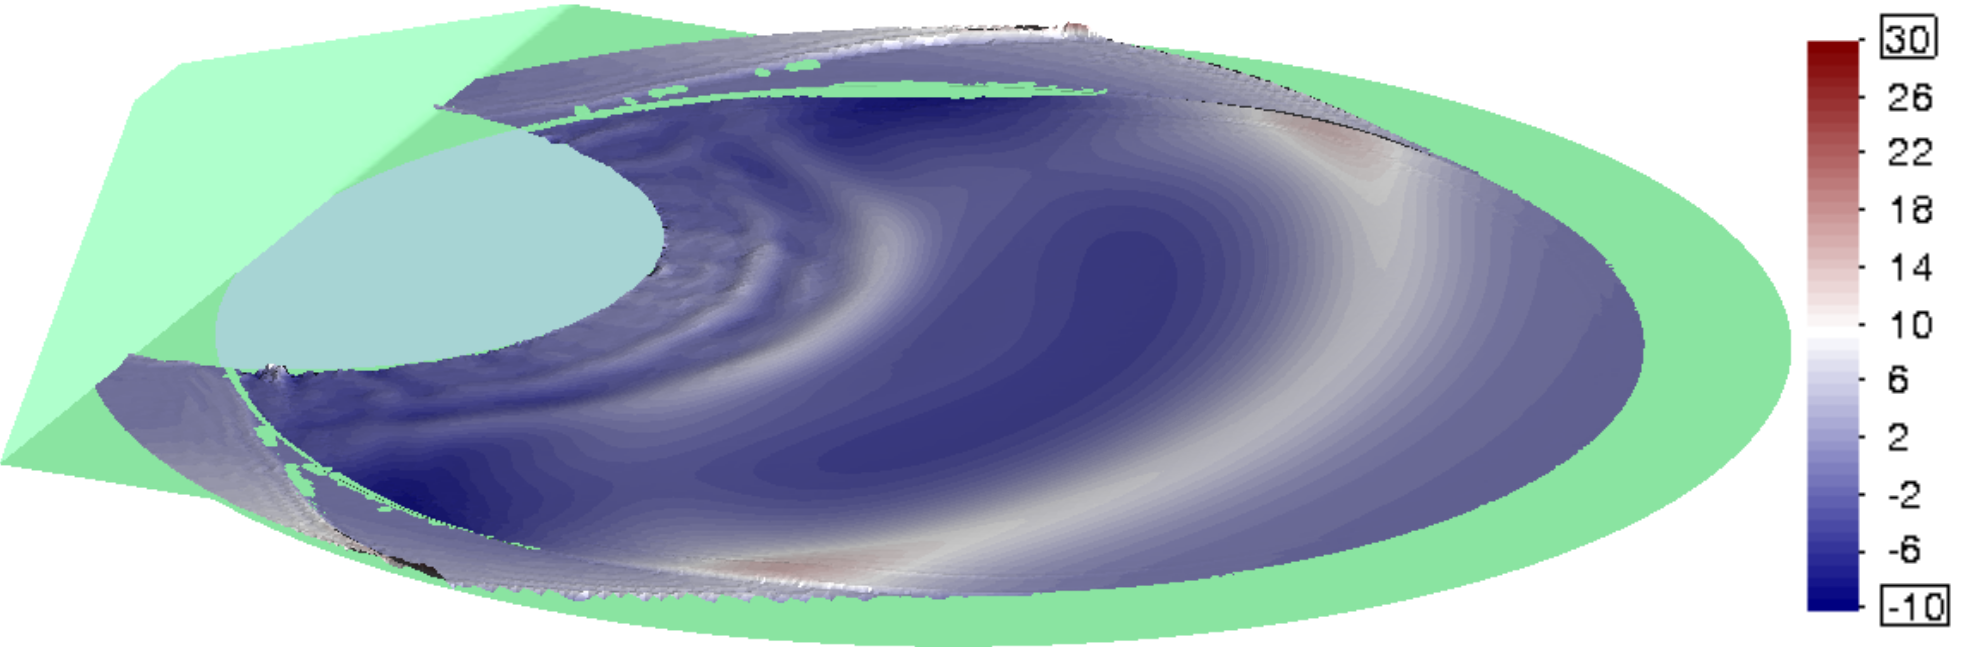
\includegraphics[width=.9\textwidth]{img/coupling/ex3_t50.png}
    \end{subfigure}
    \caption{Landslide in a representative lake. Global representation of the LGW. The NFS domain is plotted until the SW interface and only the geometry is shown. For the FFS, results for the free surface elevation are depicted.}
    \label{ex3_postprocess}
\end{figure}


In order to assess the quality of the obtained solution, in Fig. \ref{ex3_max_wave_height} we compare the envelope of the maximum wave height measured along sections $S1$ and $S2$ with the reference solution given in \cite{app112411614}.

\begin{figure} [ht]
    \centering
    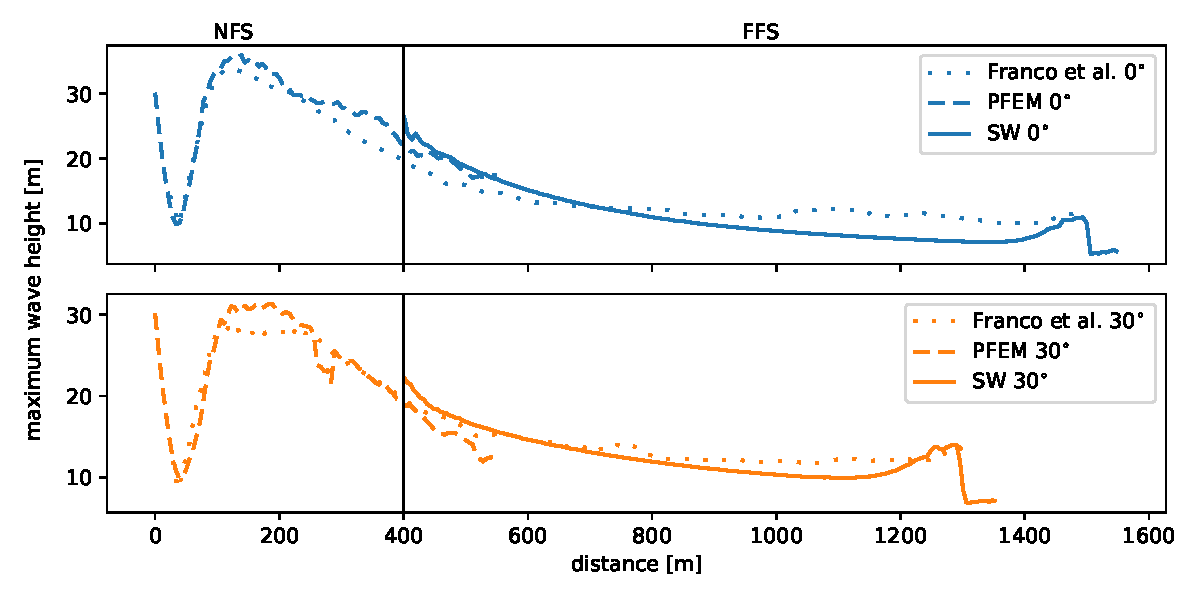
\includegraphics[width=\textwidth]{img/coupling/ex3_max_wave_height.pdf}
    \caption{Landslide in a representative lake. Envelope of the free-water-surface elevation along sections S1 and S2.}
    \label{ex3_max_wave_height}
\end{figure}

Globally, the results obtained with the proposed method agree well with the reference numerical solution, both in the near and far fields. Although with some differences in terms of magnitude, both methods are also able to reproduce the amplification of the wave near the shoreline. This phenomenon is produced by the combined effect of shoaling and the wave reflection given by the steep bottom surface. 

We also highlight that the results of the FFS are in good agreement with wave propagation theory. In an unconstrained plane, the wave amplitude is inversely proportional to the distance from the origin. Section S1 is closer to the unconstrained decay, while section S2 shows a smaller decay since it is closer to the boundary.

Finally, it is worth commenting on the peaks in amplitude exhibited by the FFS solution close to the SW interface. As mentioned before, the imposed signal coming from the PFEM simulation is still not fulfilling the Boussinesq theory. On the other hand, the generation of stable waves by Dirichlet boundary conditions requires some traveling distance to be modulated by the fluid system \cite{wu2018}. For this reason, the wave amplitude results obtained close to the SW interface with the FFS should be disregarded. We emphasize again that, on the other hand, the overall momentum computed in that zone is still correct.

In any case, the presented partitioned approach would be really interesting for an exercise like the lakes classification in \cite{app112411614}. Indeed, a single landslide calculated with the NFS could be used to simulate different representative lakes with the FFS. Also, in a more detailed study it would allow concentrating the computational resources in the analysis of the run-out and wave generation, thus enhancing the overall accuracy of the partitioned scheme.



% \clearpage
\section{Concluding remarks}

%We presented a novel partitioned strategy for solving landslide-generated wave (LGW) problems. The coupled method makes interact a near-field solver (NFS) with a far-field one (FFS). The NFS reproduces the landslide runout and the impact zone by solving the Navier Stokes equations with the Lagrangian Particle Finite Element Method (PFEM). On the other hand, the FFS uses as input the NFS results stored at a certain interface to model the wave propagation with an Eulerian Finite Element Method (FEM) based on Boussinesq shallow water (SW) equations. To improve substantially the computational performance of the method and, thus, to allow for the simulation of large-scale problems, we adopt a one-way coupling scheme, meaning that the NFS solution is insensitive to the FFS one. This partitioned method also allows us to freely decouple the time and space discretizations of the two solvers, giving a further advantage in terms of accuracy and efficiency.

In all the examples presented, the results obtained with the new partitioned method had shown a very good agreement with the reference solutions, both in 2D and 3D problems. Remarkably, we have been able to compare our numerical results with analytical solutions, fully-resolved numerical simulations of LGW events, other coupled methods presented in the literature, and experimental observations. 

Placing the SW interface as close as possible to the impact zone gives the major advantage of reducing the NFS domain and, consequently, the overall computational cost of the analysis. For this reason, we have compared the FFS results obtained considering different positions of the SW interface for the same NFS solution. This study showed that, as long the momentum of the NFS is well transferred to the FFS, the SW interface can be also placed very close to the impact zone, even if the wave is not already formed.
More specifically, the SW interface can be placed at one wavelength from the impact zone.
In fact, although locally the FFS results may give spurious amplitudes since the input wave is not fulfilling the Boussinesq theory, the stored momentum is correct and the far-field wave propagation is reproduced accurately. We remark that this can be easily done in case of having the same density between the sliding material and the water in the reservoir, such in the water landslide scenario analyzed in Section \ref{Example2}. In a more general case, the interface should be placed further than the deposition zone of the landslide, or the SW interface should take into account the variation of material densities on depth.

We have also verified the effect of reducing the size of the PFEM domain by using absorbing boundary conditions. For this purpose, a gentle final slope with an inclination of 1:10 was placed at the end of the PFEM domain. We showed that, as long as the SW interface is not placed too close to the absorbing boundary, the PFEM domain can be safely truncated without affecting the global results.
To be precise, the gentle slope should begin at least one half wavelength after the SW interface.


Finally, we also studied the effect of reducing the time duration of the NFS analyses. We have shown that, if the main interest of the simulation of the LGW scenario is to reproduce the main wave propagation, the PFEM analysis can be safely stopped after it has modeled the impact of the landslide on the water and the first wave formation. Indeed, this time truncation of the NFS will only affect the secondary waves propagation. We also showed that, knowing the NFS duration and the wave propagation speed, it is possible to have a quite accurate estimation of the reliability of the secondary waves results. 
 
All these specific studies will allow us the define the most computational efficient NFS-FFS scheme for practical LGW simulations.  Although the overall computational cost depends inevitably on the geometry and the proportions among the near and far fields, in the examples here presented, we could estimate a $90\%$ of time saving versus a fully-resolved simulation of the same LGW scenario.


Among the possible enhancements of the proposed method, we consider it of primary interest to investigate more efficient strategies for the NFS absorbing boundaries and to develop a reverse one-way coupled algorithm where the FFS transfers the information to the NFS. This FFS-NFS model would allow us simulating with high accuracy the effect of tsunami waves produced by landslides (or by some other source, $i.e.$, an earthquake) on the shoreline and the civil constructions placed therein.

